\section{Life Cycle Assessment: Aaron Li}
\label{sec:lca}

\subsection{Methodology}

Life Cycle Assessment (LCA) was conducted following ISO 14040 to compare the environmental impacts of the reference product (current disposable e-cigarette design) to a DfD-redesigned concept.

\textbf{Software}: Sustainable Minds

\textbf{Functional unit}: 1000 disposable e-cigarette devices delivering $\sim$3{,}000 puffs of nicotine aerosol (Air Bar NEX 3K rated capacity).

\textbf{System boundary}: Cradle-to-grave, including:

\begin{itemize}
    \item Raw material extraction and processing
    \item Manufacturing and assembly
    \item Transportation (manufacturing site to point of sale)
    \item Use phase (negligible environmental impact beyond embodied energy)
    \item End-of-life (landfill for reference; recycling pathway for DfD concept)
\end{itemize}

\subsection{Simplified Bill of Materials (SBOM)}

\begin{table}[H]
\centering
\caption{Simplified Bill of Materials for LCA input.}
\label{tab:sbom}
\begin{tabular}{@{}llr@{}}
\toprule
\textbf{Component} & \textbf{Material (LCI Entry)} & \textbf{Mass (g)} \\
\midrule
Battery cell (13450) & Lithium-ion battery, rechargeable (3.7\,V, 650\,mAh) & 12.0 \\
Housing              & Aluminium, wrought alloy (anodized) & 13.0 \\
PCB assembly         & Printed circuit board, surface mounted & 2.0 \\
Atomizer coil + wick & Kanthal/nichrome wire, cotton & \multicolumn{1}{c}{incl.\ below} \\
Mouthpiece           & Polypropylene, injection molded & \multicolumn{1}{c}{---\textsuperscript{a}} \\
E-liquid reservoir (incl.\ atomizer) & Cotton fibre, plastic absorbent, e-liquid & 10.0 \\
Inner chassis, seals, wires & PC/ABS, silicone rubber, copper wire & \multicolumn{1}{c}{---\textsuperscript{a}} \\
\midrule
\textbf{Total}       & & 52.0 \\
\bottomrule
\end{tabular}
\end{table}

\noindent\textsuperscript{a} Mouthpiece, inner chassis, seals, and wires were not individually weighed. Combined remainder: $52.0 - 12.0 - 13.0 - 2.0 - 10.0 = 15.0$\,g.

\subsection{Reference Product LCA (Current Design)}

To produce the reference product LCA, we took the measured values of the part components listed in the bill of materials  and, to the best of our ability, entered them into the Sustainable Minds software.  Some parts such as nichrome and FR4 were not defined in the software, so those were broken down into their elemental percentages and entered the system.   The transportation was accounted for the typical travel distance from the manufacturers in China to a seller in New York, a distance of 6000 miles.  For the purposes of the reference, all the components possible were sent to landfill.  Also accounted for were the typical 3 recharges before disposal, each of which at 0.005 kWh. 

\begin{figure}[H]
    \centering
    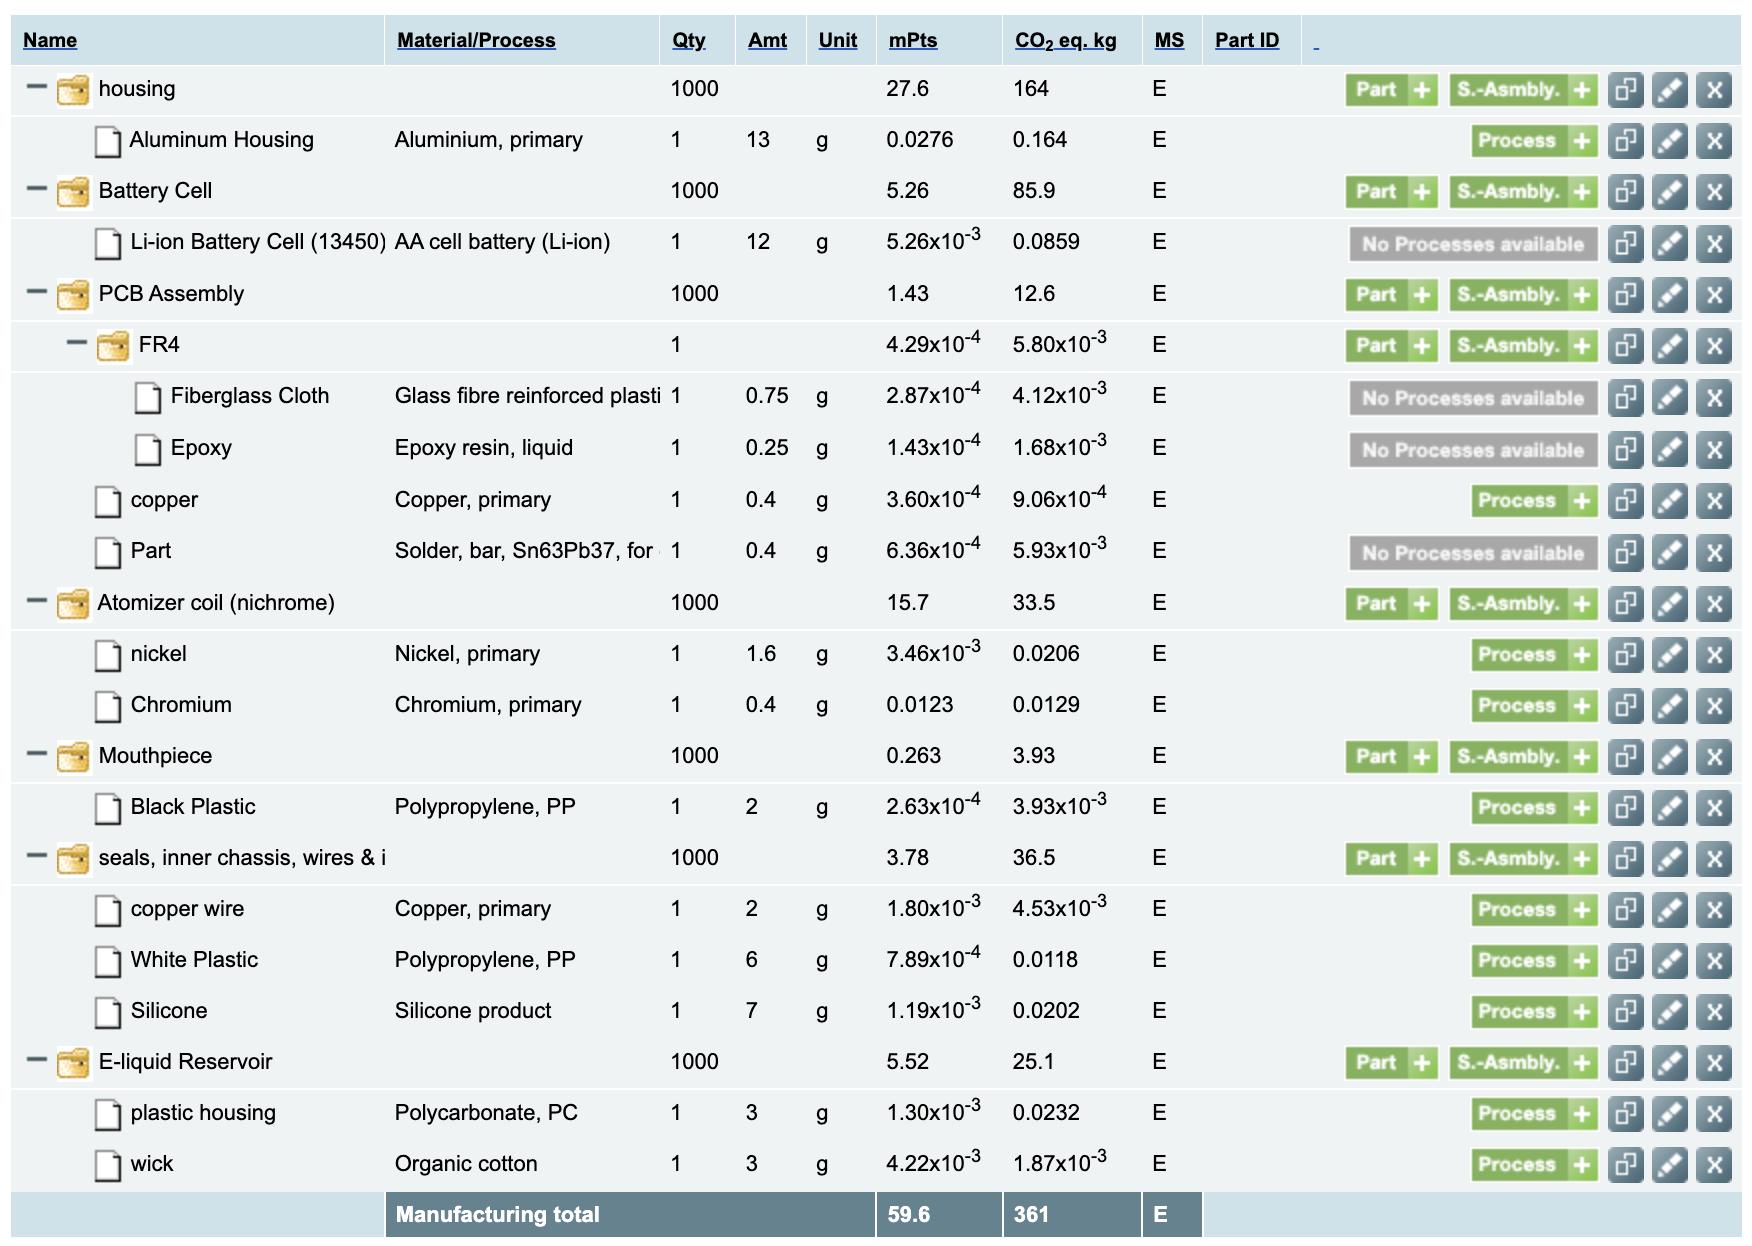
\includegraphics[width=0.7\linewidth]{Screenshot 2026-03-11 at 7.17.48 PM.png}
        \caption{System BOM for Reference Air Bar}
    \label{fig:placeholder}
\end{figure}
\begin{figure}[H]
        \centering
        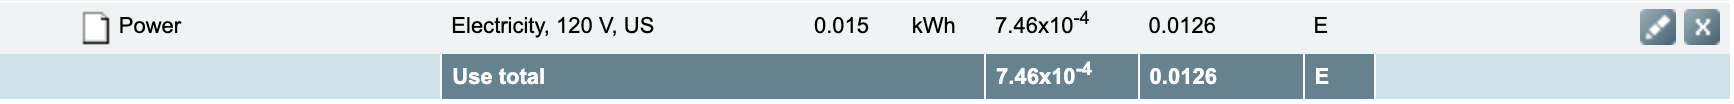
\includegraphics[width=0.75\linewidth]{Screenshot 2026-03-11 at 8.16.47 PM.png}
        \caption{Energy Use}
        \label{fig:placeholder}
\end{figure}
\begin{figure}[H]
    \centering
    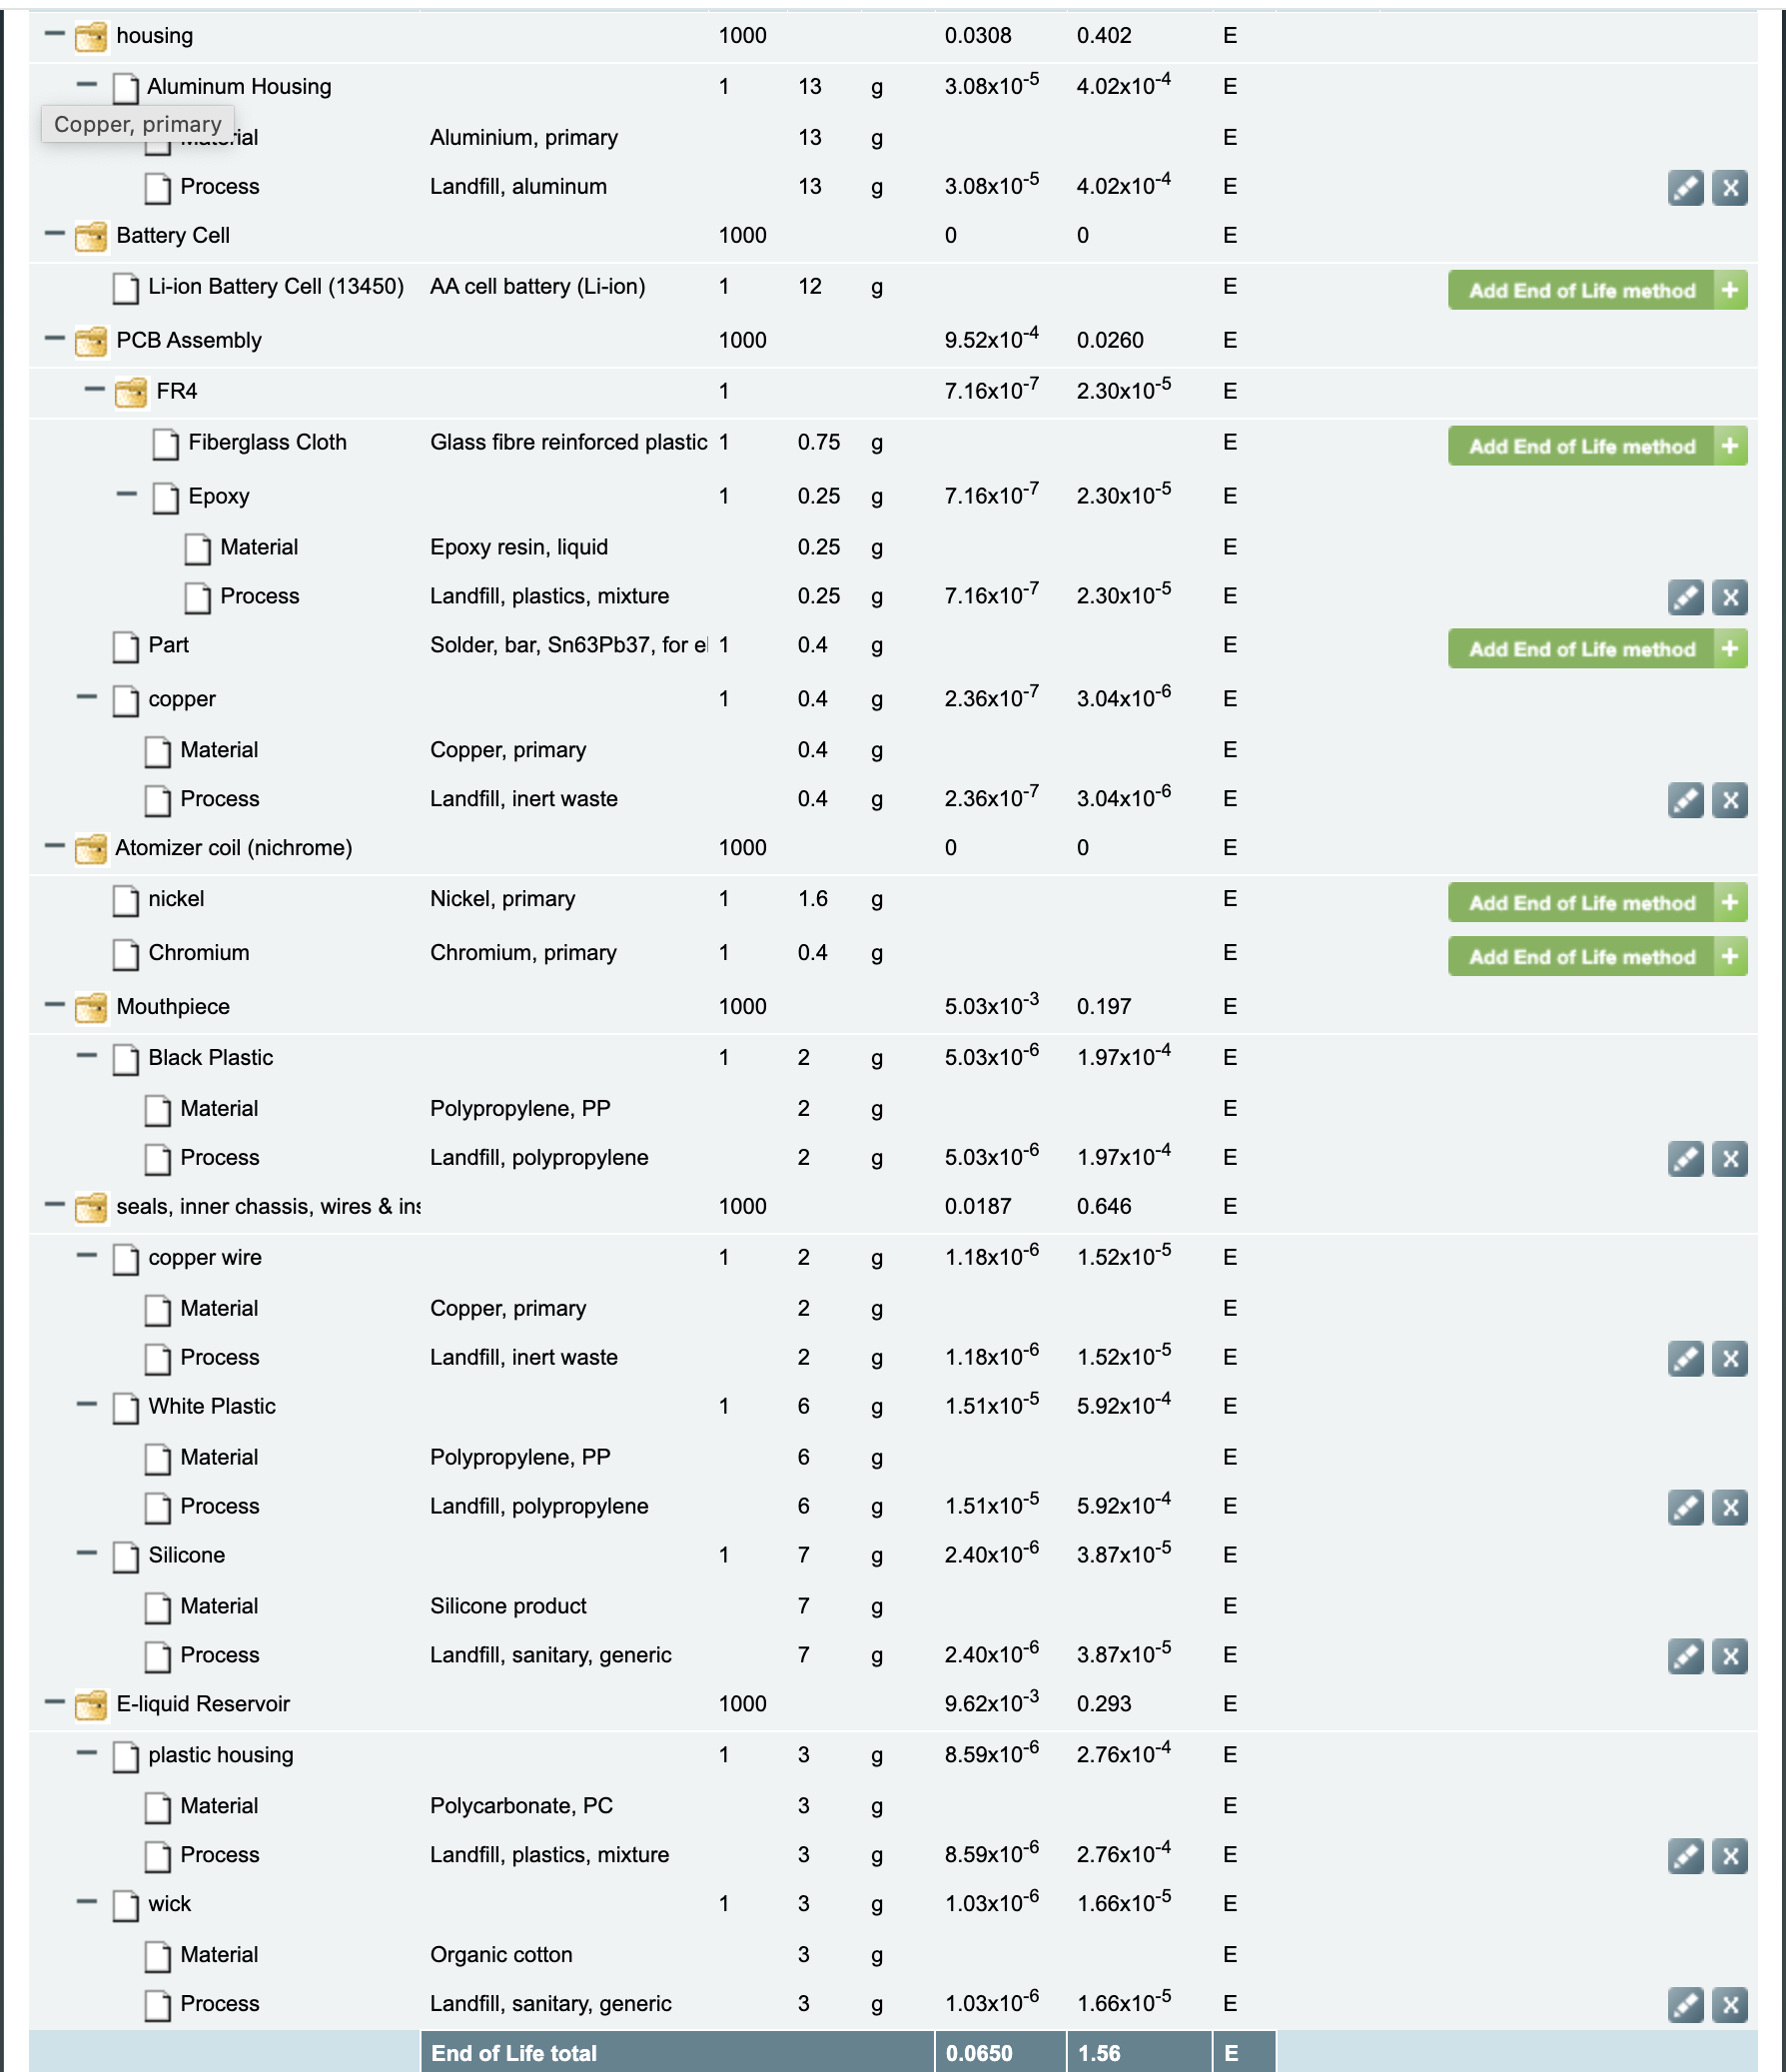
\includegraphics[width=0.75\linewidth]{Screenshot 2026-03-11 at 7.58.01 PM.png}
    \caption{End of Life Analysis for Reference}

        \label{fig:placeholder}
\end{figure}
\begin{figure}[H]
    \centering
    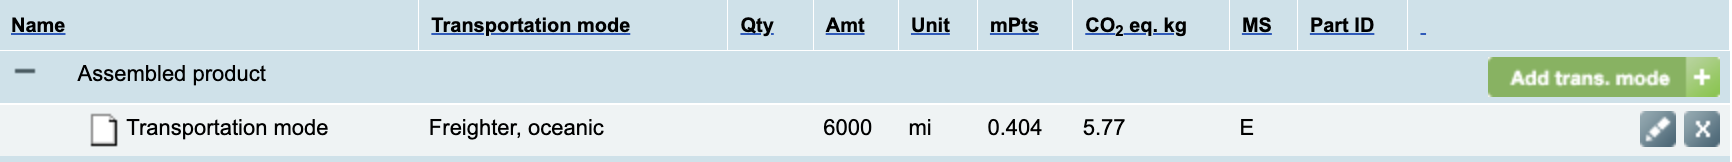
\includegraphics[width=0.75\linewidth]{Screenshot 2026-03-11 at 8.06.03 PM.png}
    \caption{Transportation Analysis for Reference}
    \label{fig:placeholder}
\end{figure}
\subsubsection{Impact Categories}

\begin{figure}[H]
    \centering
    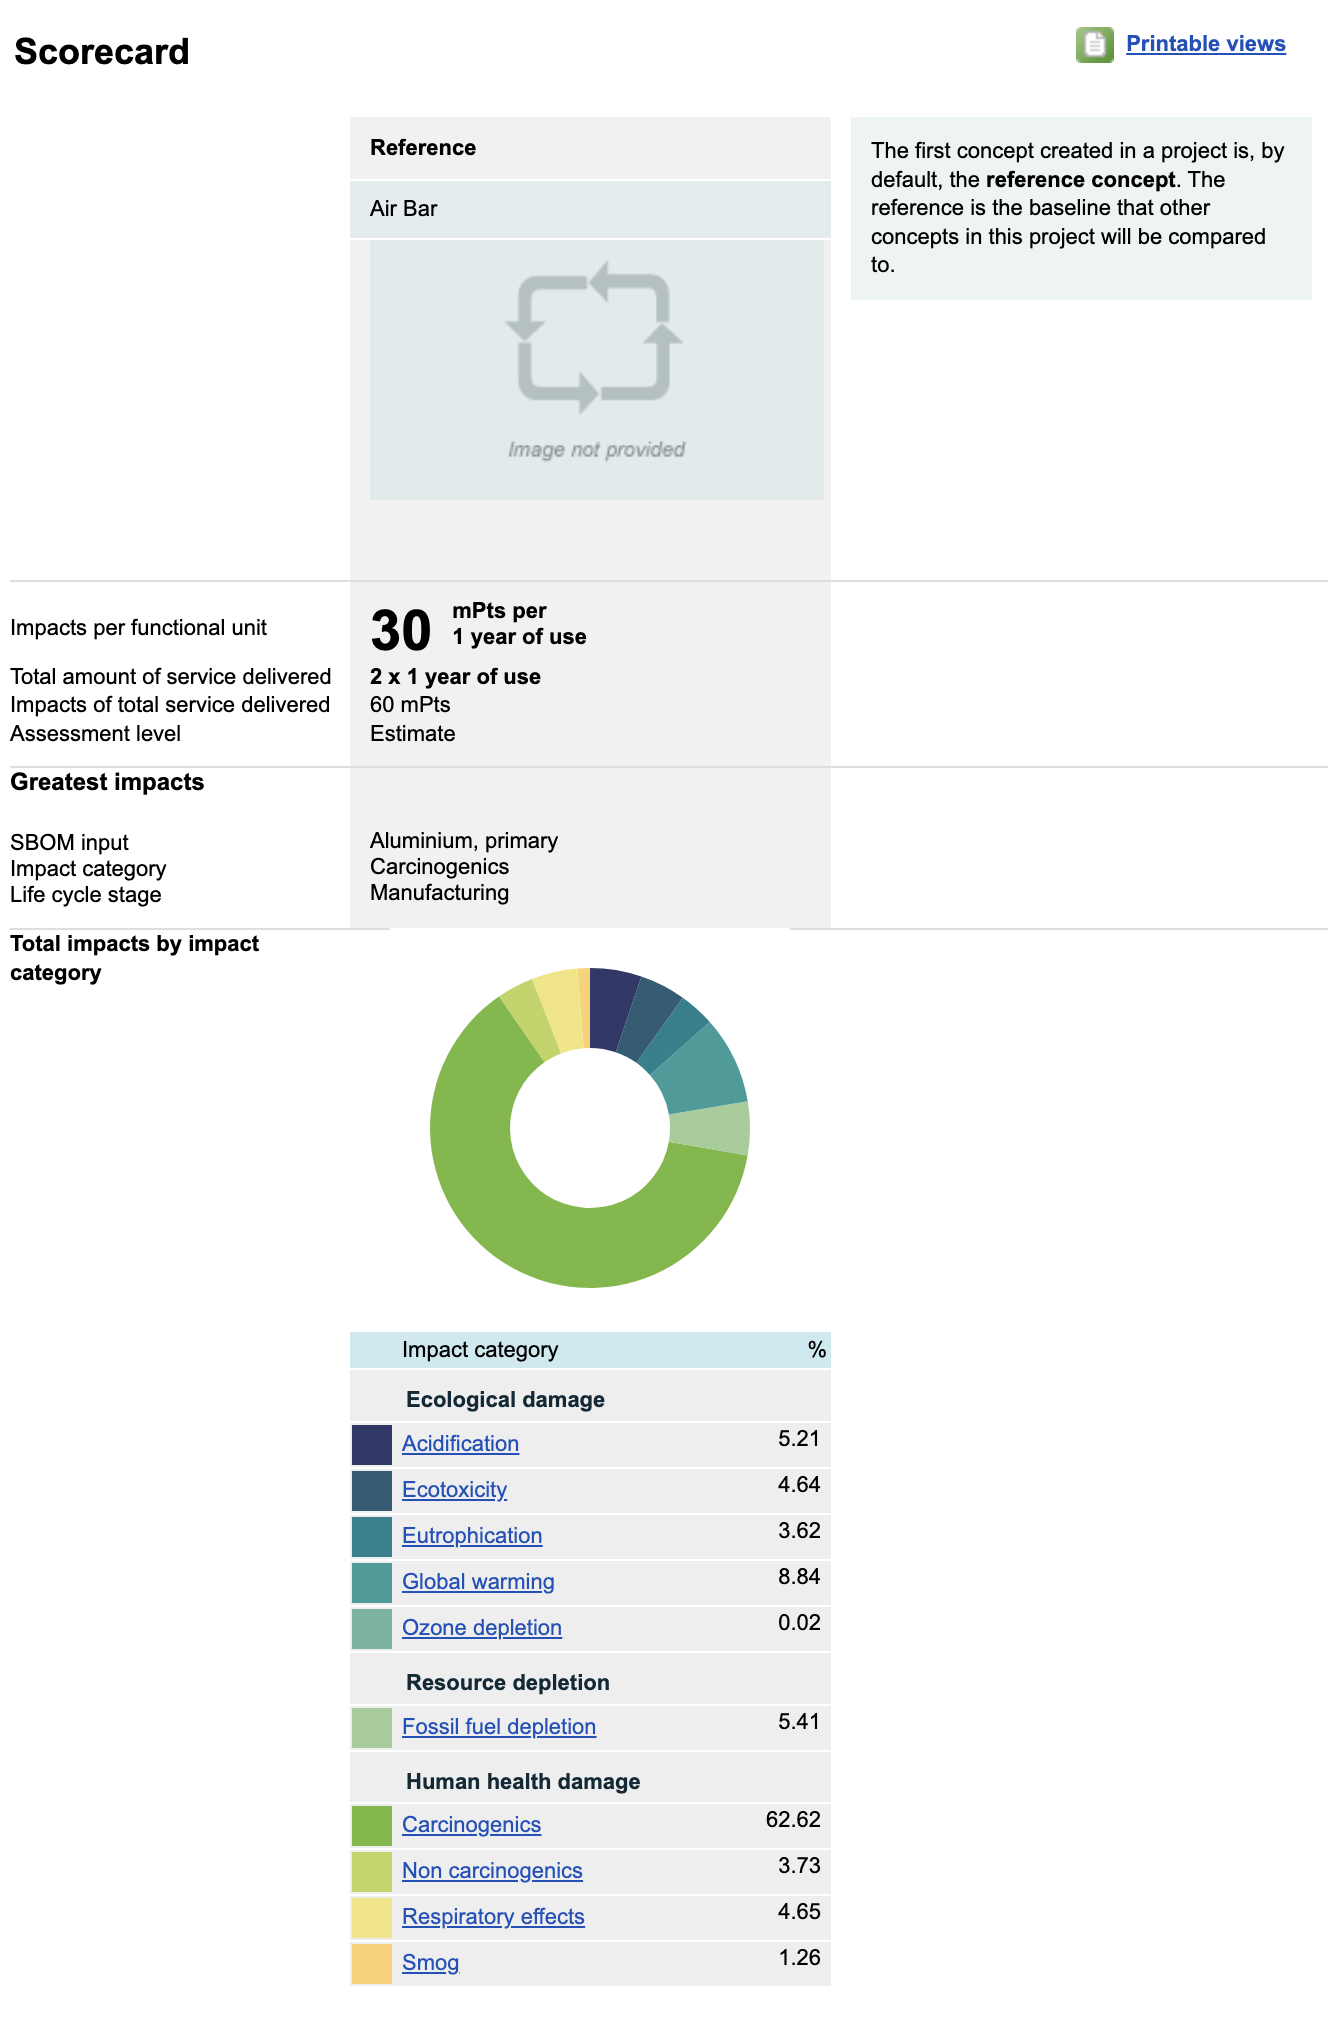
\includegraphics[width=0.75\linewidth]{Screenshot 2026-03-11 at 7.33.51 PM.png}
    \caption{Impact Categories}
    \label{fig:placeholder}
\end{figure}

\subsubsection{Impacts by SBOM Inputs}
\begin{figure}[H]
    \centering
    \begin{subfigure}{0.42\textwidth}
        \centering
        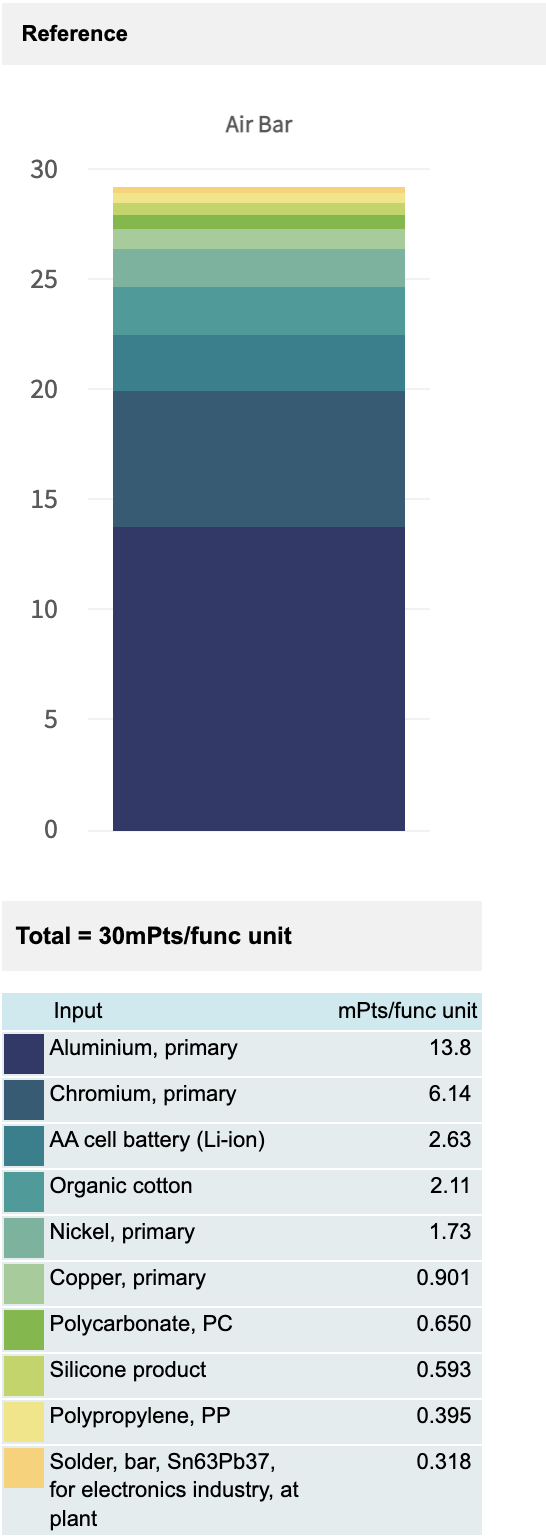
\includegraphics[width=\linewidth]{Screenshot 2026-03-11 at 7.41.08 PM.png}
        \caption{Impacts on mPts based on SBOM}
        \label{fig:placeholder}
    \end{subfigure}
    \hfill
    \begin{subfigure}{0.42\textwidth}
        \centering
        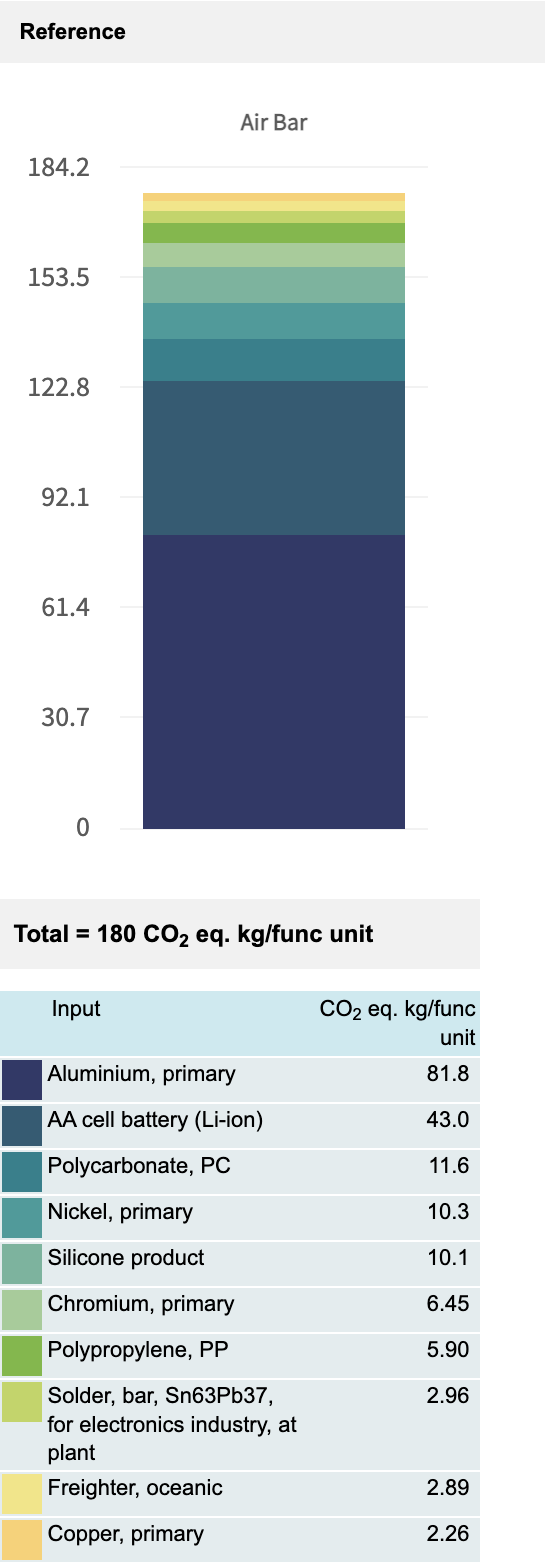
\includegraphics[width=\linewidth]{Screenshot 2026-03-11 at 7.41.24 PM.png}
        \caption{Carbon Footprint of SBOM components}
        \label{fig:placeholder}
    \end{subfigure}
\end{figure}
\subsubsection{Life Cycle Stage Breakdown}

\begin{figure}[H]
    \centering
    \begin{subfigure}{0.42\textwidth}
        \centering
        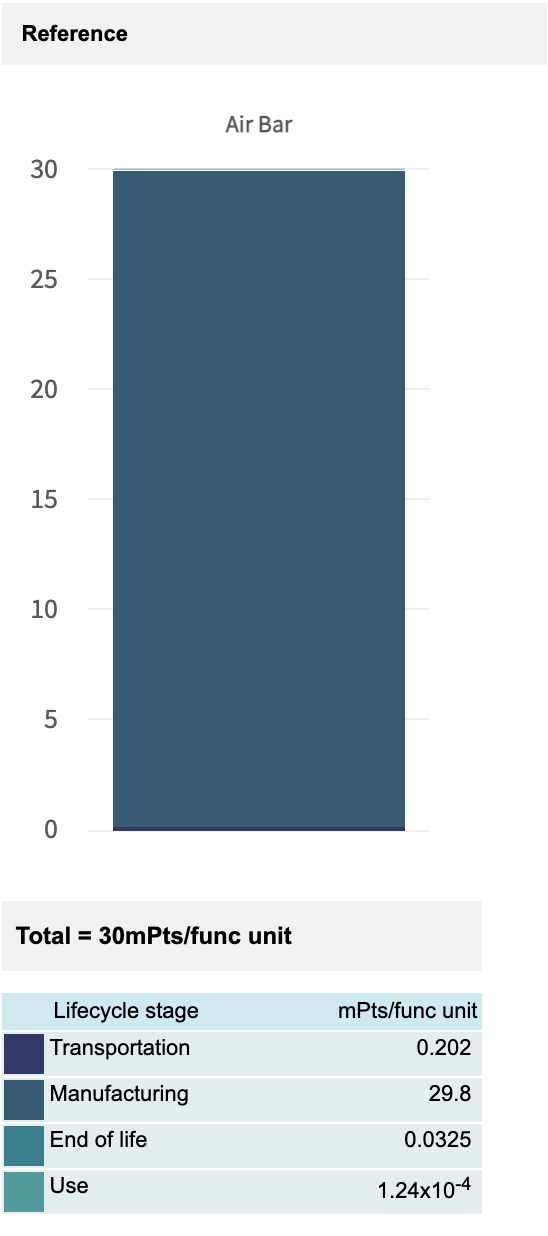
\includegraphics[width=\linewidth]{Screenshot 2026-03-11 at 7.48.56 PM.png}
        \caption{Total Impact by Life Cycle}
        \label{fig:placeholder}
    \end{subfigure}
    \hfill
    \begin{subfigure}{0.42\textwidth}
        \centering
        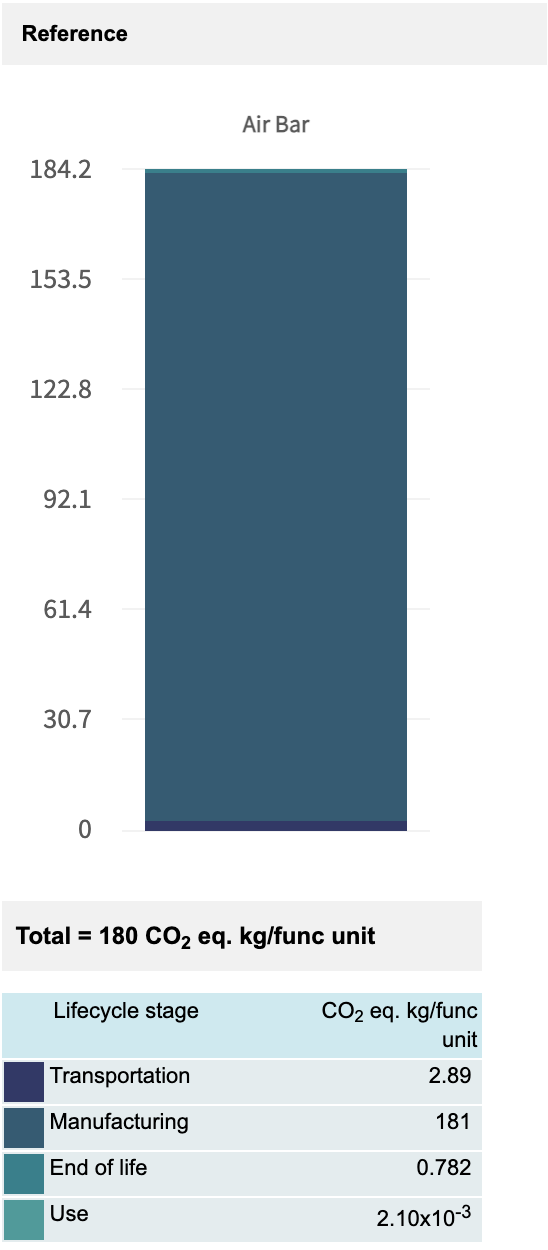
\includegraphics[width=\linewidth]{Screenshot 2026-03-11 at 7.49.05 PM.png}
        \caption{Carbon Footprint Impact by Life Cycle}
        \label{fig:placeholder}
    \end{subfigure}
\end{figure}
% \begin{figure}[H]
%     \centering
%     \includegraphics[width=0.9\textwidth]{figures/lca_reference_breakdown.pdf}
%     \caption{Life cycle stage contribution to environmental impacts --- reference product.}
%     \label{fig:lca_reference}
% \end{figure}

\subsection{DfD Concept LCA}

After analyzing the information from the results of the reference Air Bar, we determined that contrary to what we initially believed, a significant contributor to environmental impact was the manufacturing.  In this new design, we aimed to make changes to components of the product that would be much more sustainable, all while maintaining the functionality of the product.  As the manufacturing of the product would take place in China and be shipped to New York, the method of transportation being oceanic freight was already optimized.  The end-of-life method was changed from landfill to recycling to benefit the impact from the end of the life cycle.  Due to the new snap fit design, we predict that the amount of E-liquid refills will increase, meaning more recharges.  This accounts for around 100 recharges instead of 3.  Most of the other components like the plastics, the wick, battery, and other electronic components are already optimized for the functionality of the product, and were thus not changed.  
\begin{figure}[H]
    \centering
    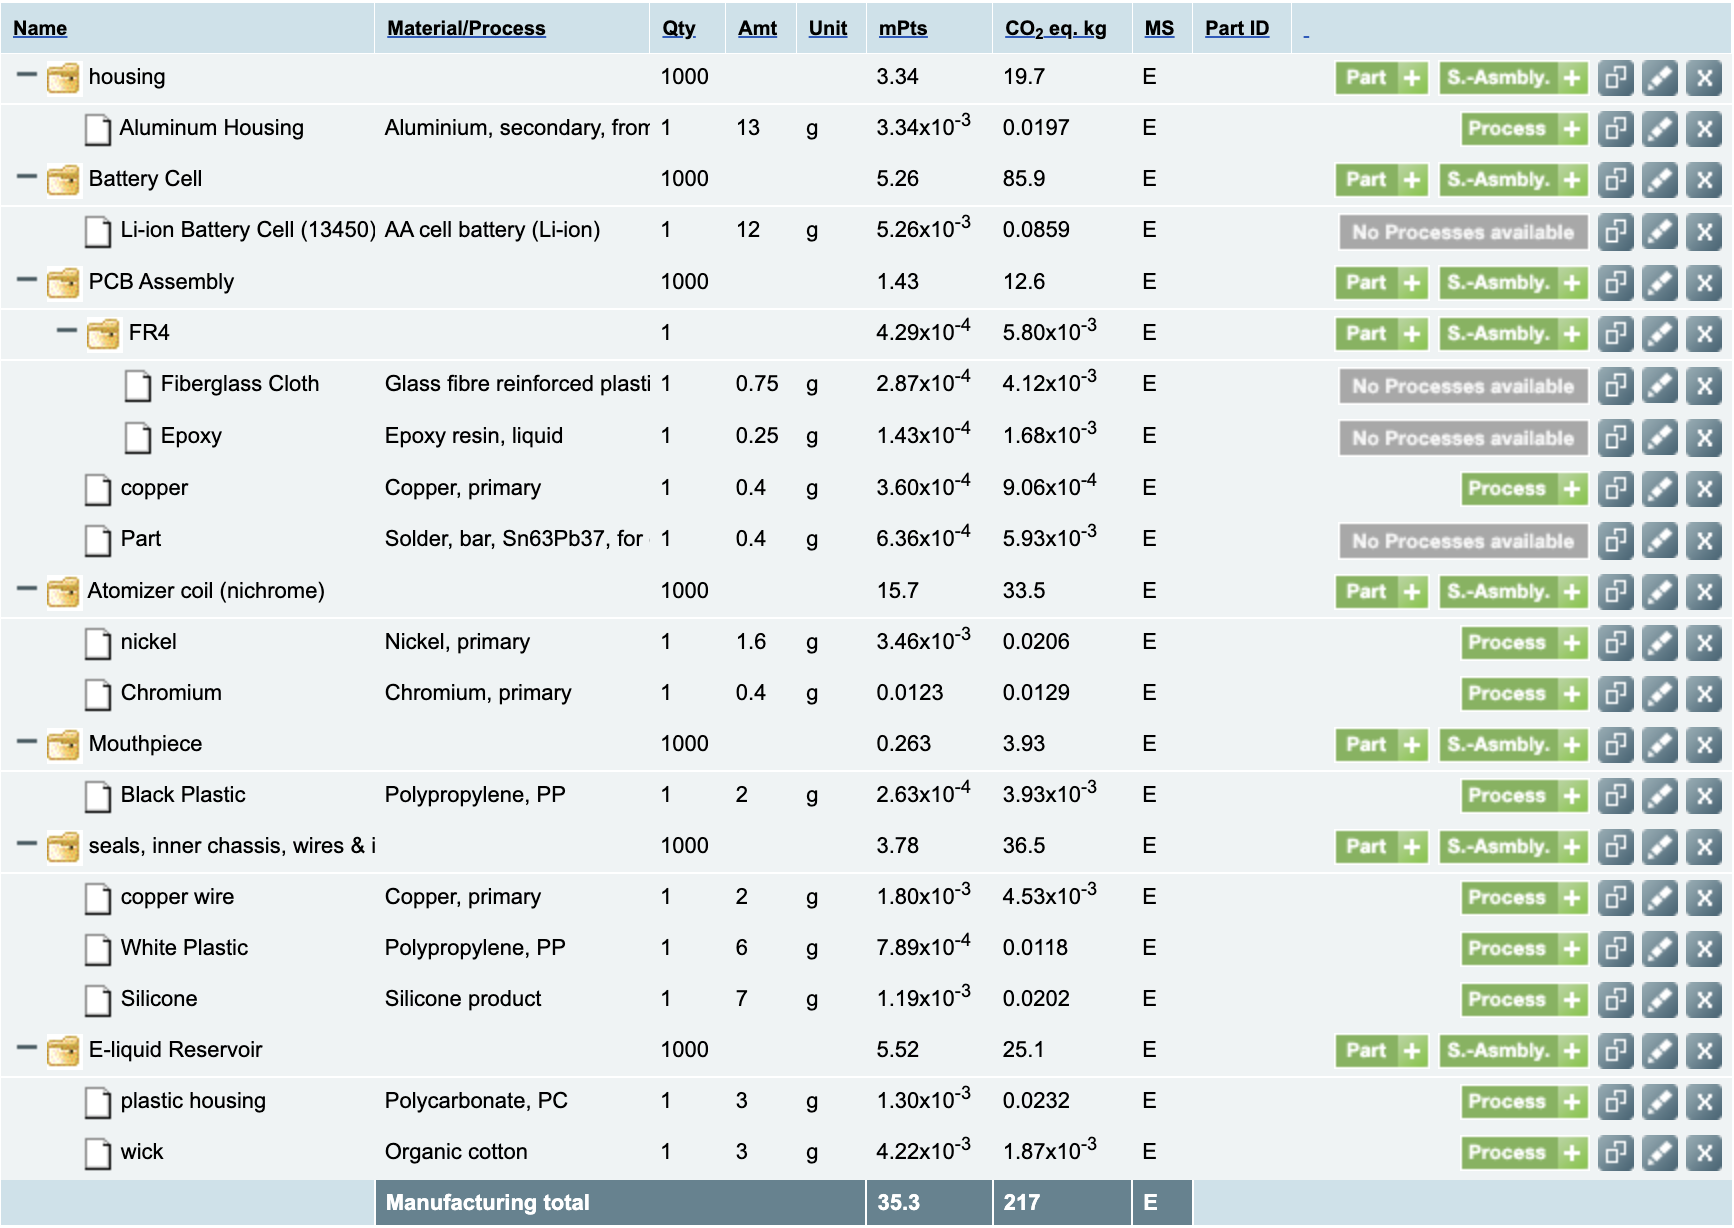
\includegraphics[width=0.65\linewidth]{Screenshot 2026-03-11 at 8.25.16 PM.png}
    \caption{System SBOM for New Air Bar}
    \label{fig:placeholder}
\end{figure}
\begin{figure}[H]
    \centering
    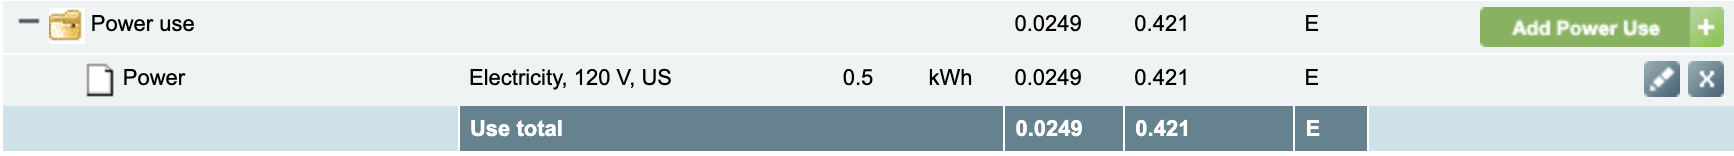
\includegraphics[width=0.65\linewidth]{Screenshot 2026-03-11 at 8.25.39 PM.png}
    \caption{Energy Use of New}
    \label{fig:placeholder}
\end{figure}
\begin{figure}[H]
    \centering
    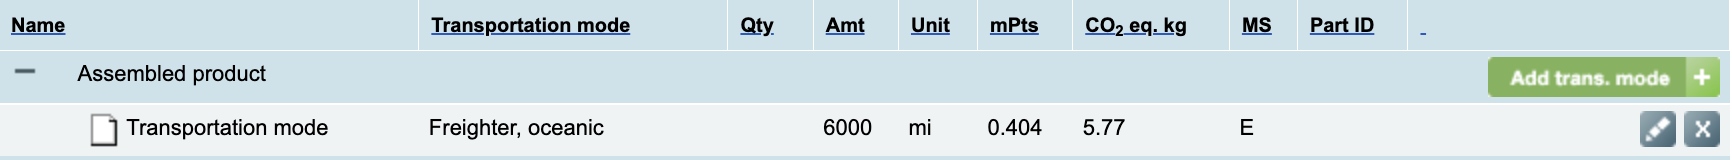
\includegraphics[width=0.65\linewidth]{Screenshot 2026-03-11 at 8.35.11 PM.png}
    \caption{Transportation for New}
    \label{fig:placeholder}
\end{figure}
\begin{figure}[H]
    \centering
    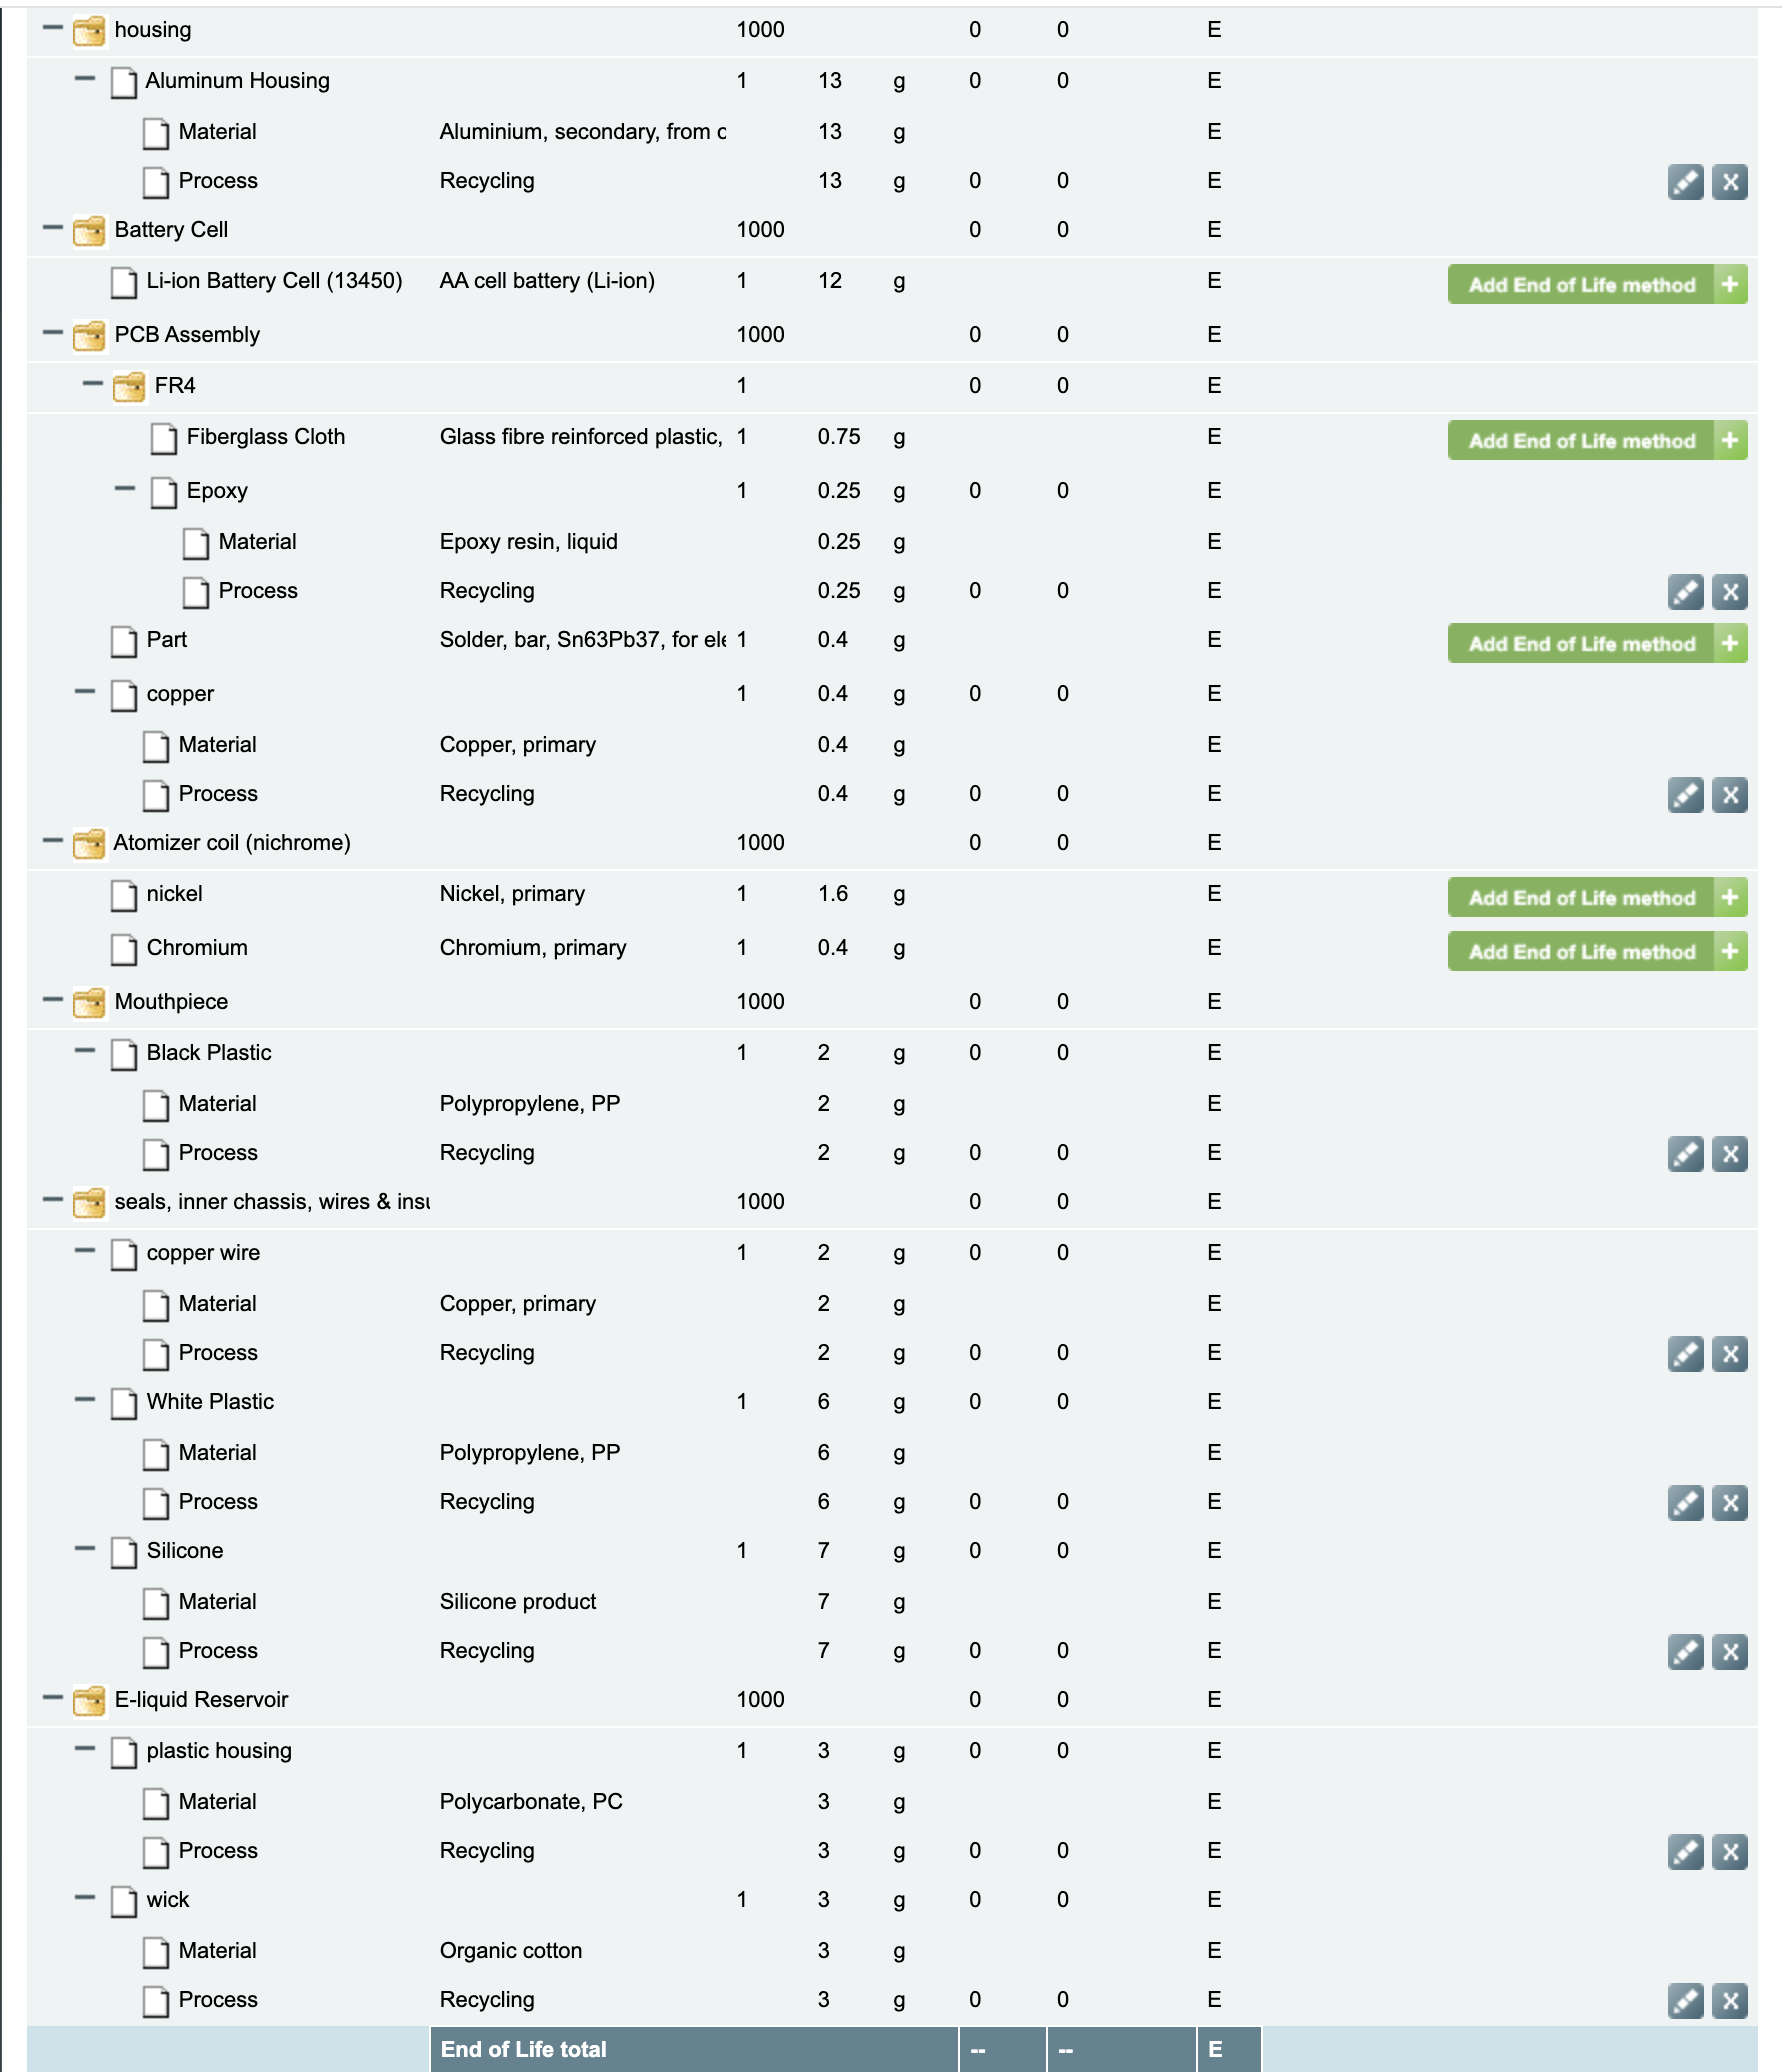
\includegraphics[width=0.65\linewidth]{Screenshot 2026-03-11 at 8.30.48 PM.png}
    \caption{End of Life Analysis for New}
    \label{fig:placeholder}
\end{figure}
\subsection{Comparison Results}

\begin{figure}[H]
    \centering
    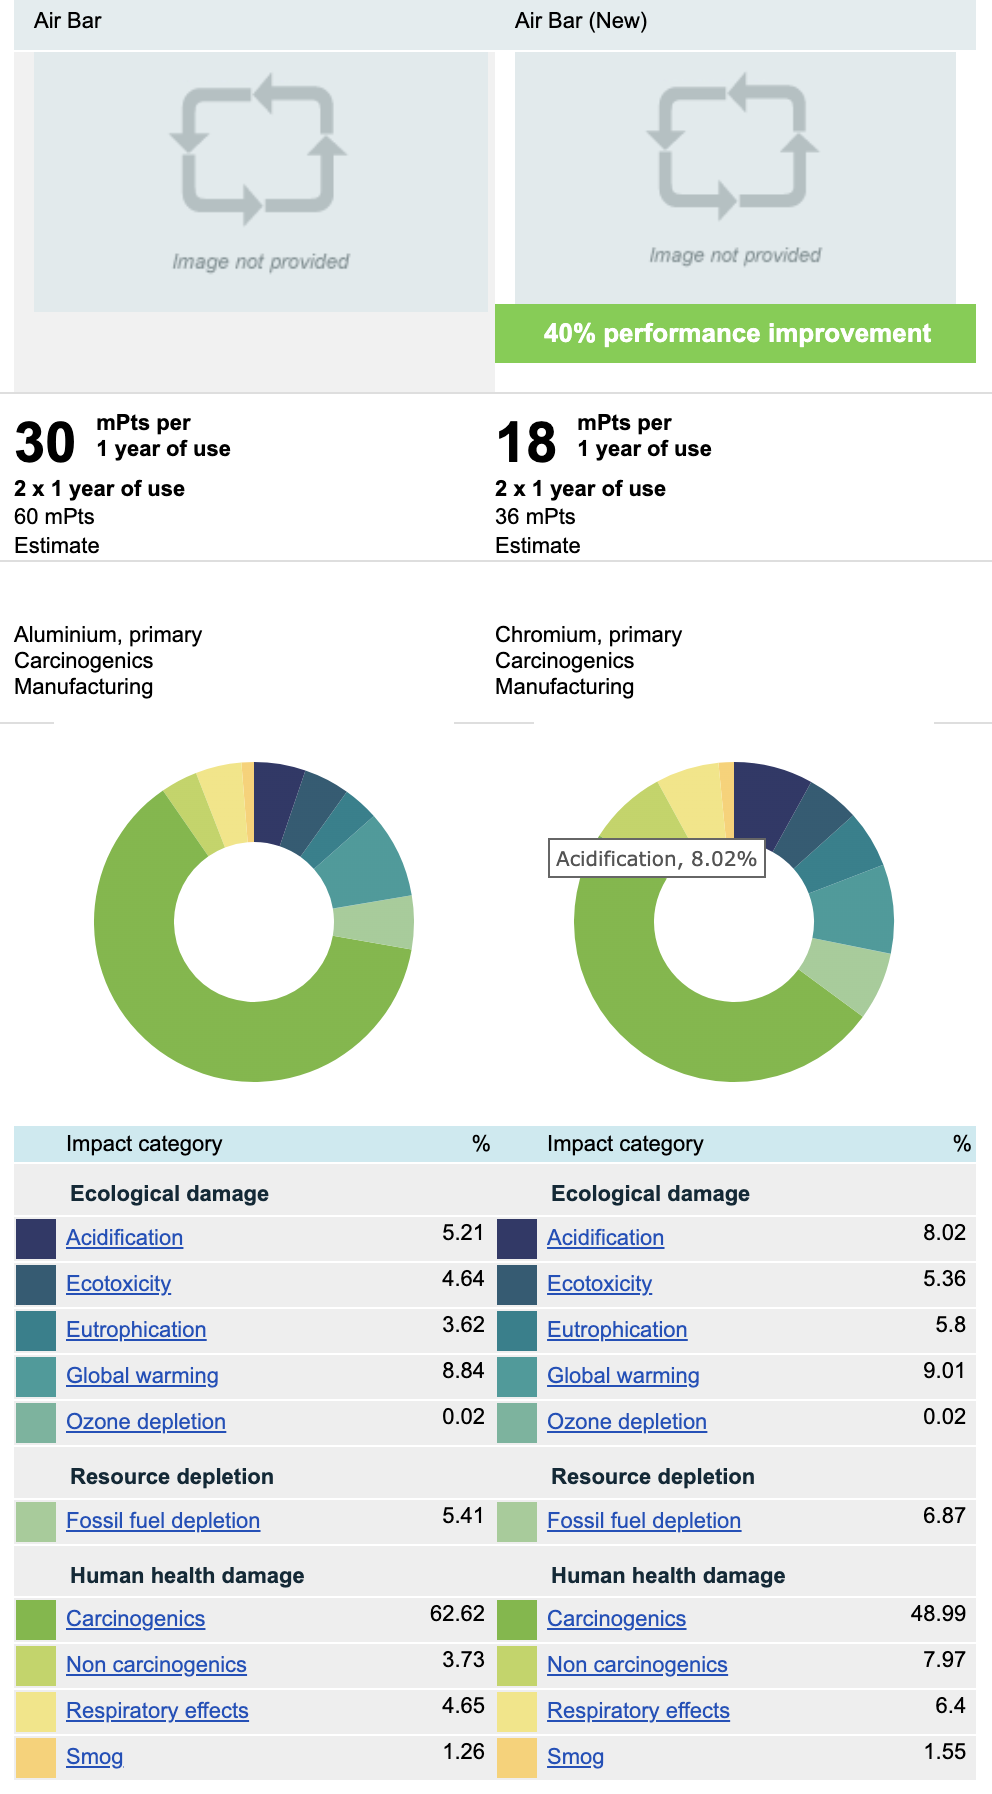
\includegraphics[width=0.5\linewidth]{Screenshot 2026-03-11 at 8.41.59 PM.png}
    \caption{Scorecard Comparison}
    \label{fig:placeholder}
\end{figure}

\begin{figure}[H]
    \centering
    \begin{subfigure}{0.48\textwidth}
        \centering
        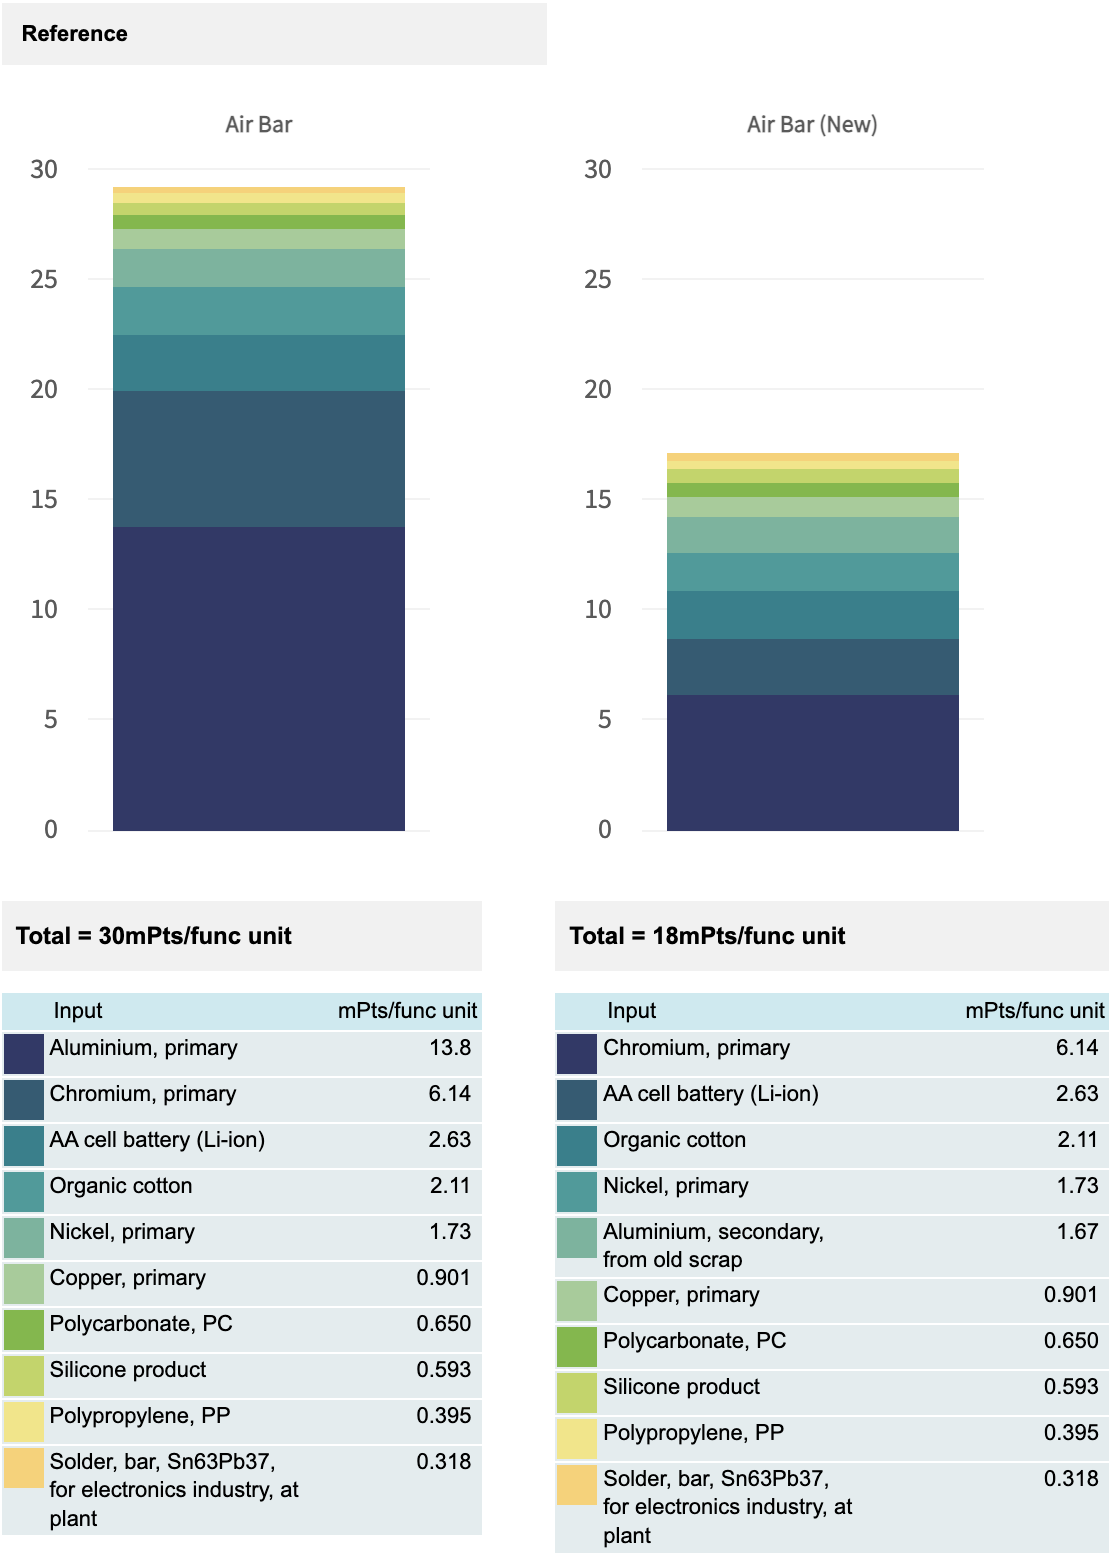
\includegraphics[width=\linewidth]{Screenshot 2026-03-11 at 8.42.49 PM.png}
        \caption{Total SBOM Impact of New Air Bar}
        \label{fig:placeholder}
    \end{subfigure}
    \hfill
    \begin{subfigure}{0.48\textwidth}
        \centering
        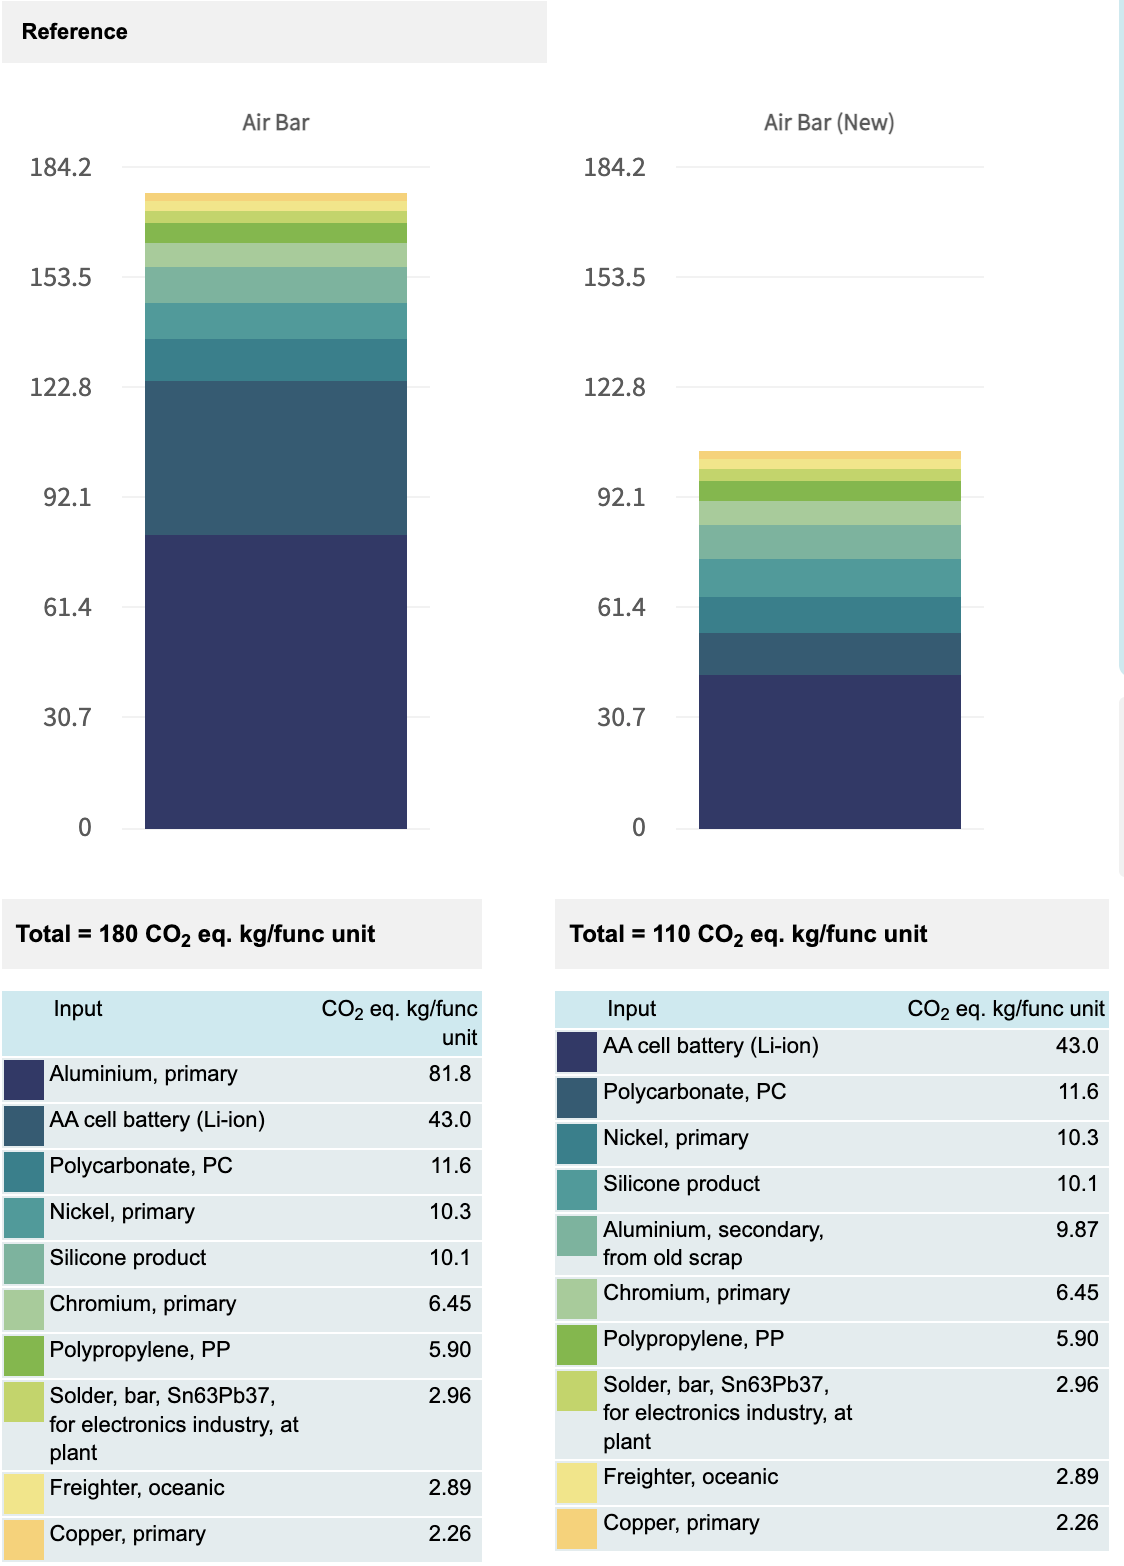
\includegraphics[width=\linewidth]{Screenshot 2026-03-11 at 8.43.32 PM.png}
        \caption{Carbon Footprint of New Air Bar SBOM}
        \label{fig:placeholder}
    \end{subfigure}
\end{figure}

\begin{figure}[H]
    \centering
    \begin{subfigure}{0.48\textwidth}
        \centering
        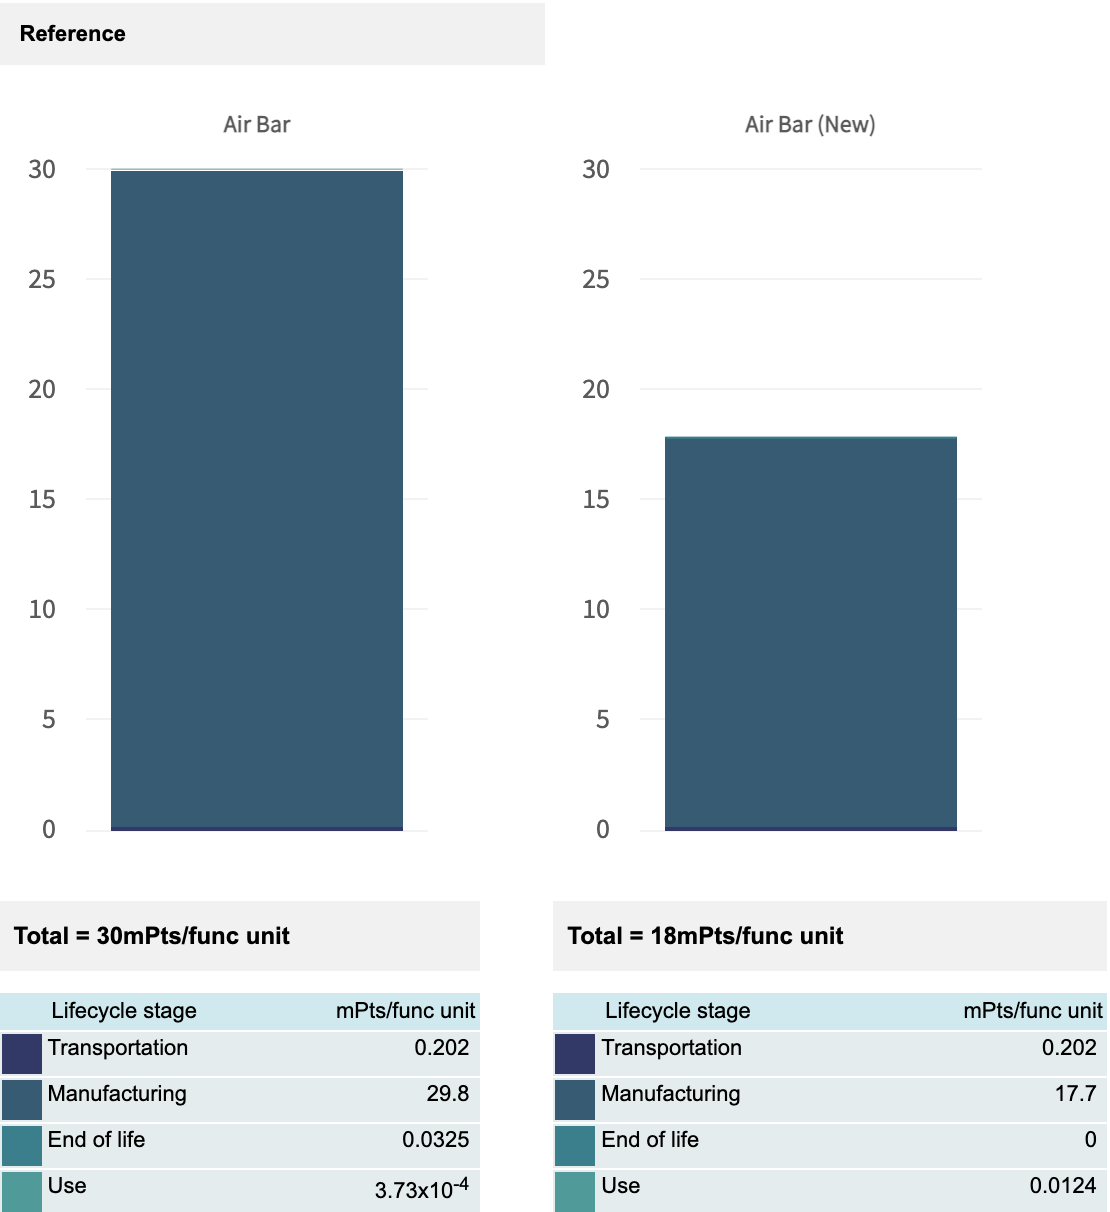
\includegraphics[width=\linewidth]{Screenshot 2026-03-11 at 8.43.45 PM.png}
        \caption{Life Cycle Analysis of New Air Bar}
        \label{fig:placeholder}
    \end{subfigure}
    \hfill
    \begin{subfigure}{0.48\textwidth}
        \centering
        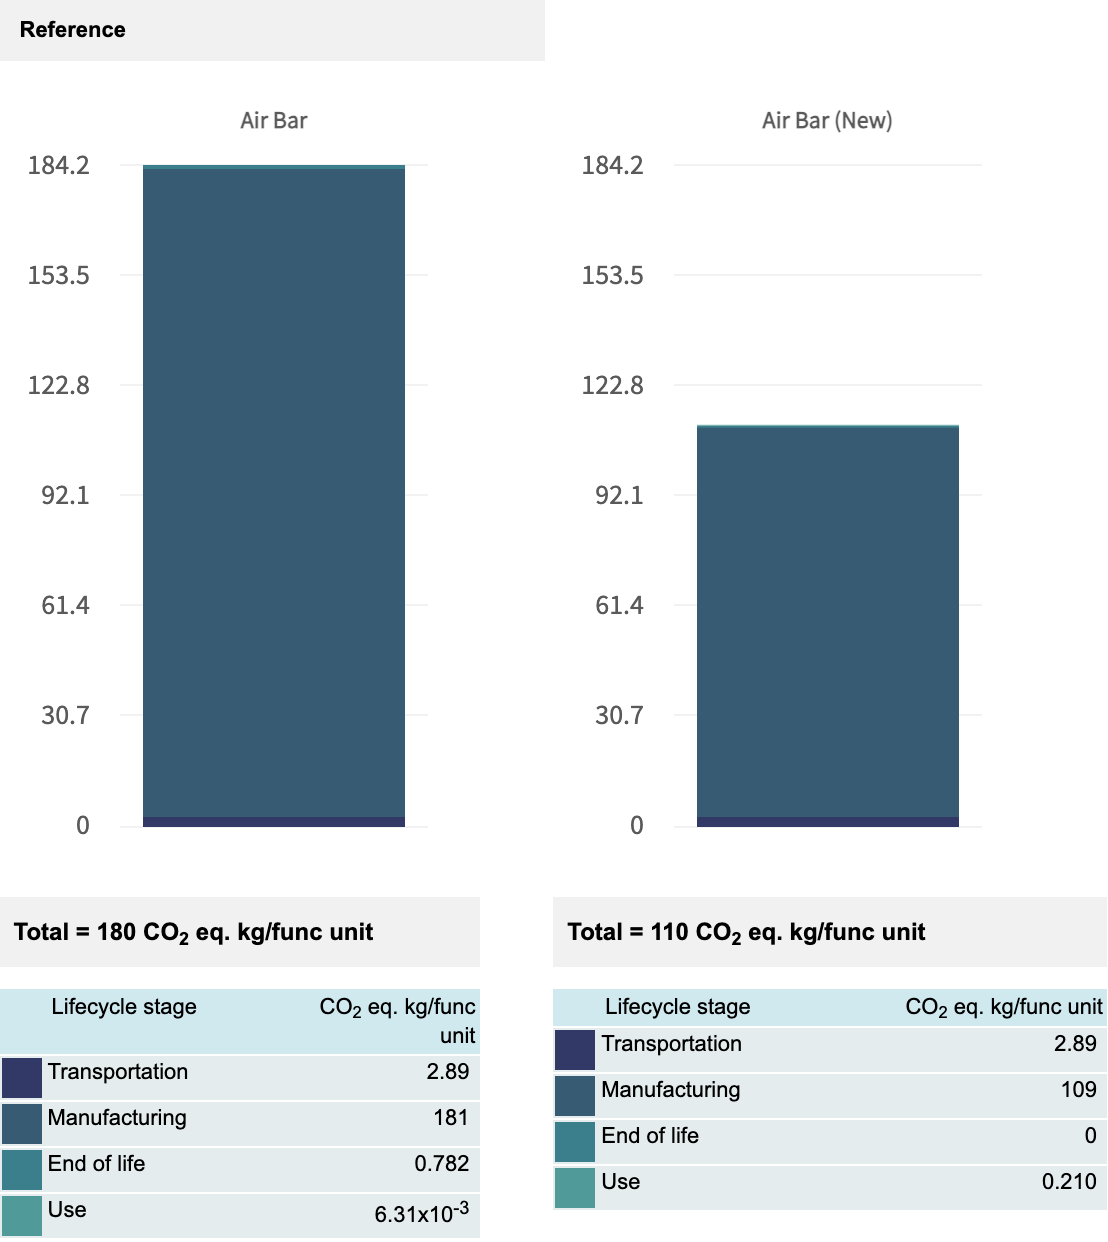
\includegraphics[width=\linewidth]{Screenshot 2026-03-11 at 8.43.57 PM.png}
        \caption{New Air Bar Carbon Footprint of Life Cycle }
        \label{fig:placeholder}
    \end{subfigure}
\end{figure}


\subsection{Identification of Greatest Impacts}

After the analysis of both the reference product and the new Air Bar, we were able to see the area of greatest impact.  Unlike what was originally believed, the greatest impact came from the change of the Aluminum housing.  Simply by changing the kind of Aluminum from primary to a secondary aluminum recycled from aluminum scraps was able to give a great decrease in environmental harm.  While we believed that changing the life-cycle factor by going from landfill to recycling, the change was not very significant.  Even after considering an increase in energy use from the more often battery recharges, those impacts were minuscule compared to the change in aluminum.  So with a new method of aluminum manufacturing for the new Air Bar housing, we can greatly decrease the environmental impact from the production of the Air Bar Vapes.  



% \begin{figure}[H]
%     \centering
%     \includegraphics[width=0.9\textwidth]{figures/lca_comparison.pdf}
%     \caption{LCA comparison: reference product vs.\ DfD concept across impact categories.}
%     \label{fig:lca_comparison}
% \end{figure}
